\textbf{Solução:}
As Figuras a seguir mostram os passos da remoção das chaves A, B, M, Q e R da árvore B do enunciado. Foi utilizada a ferramenta B-Tree Visualization\footnote{Disponível em \href{https://www.cs.usfca.edu/~galles/visualization/BTree.html}{https://www.cs.usfca.edu/~galles/visualization/BTree.html}.}, da University of San Francisco, porém apenas a título de visualização; os resultados foram feitos à mão ``no papel''.

\begin{figure}[H]
    \centering
    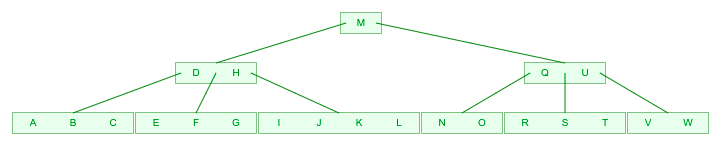
\includegraphics[width=\linewidth]{tree_1.png}
\end{figure}

\begin{figure}[H]
    \centering
    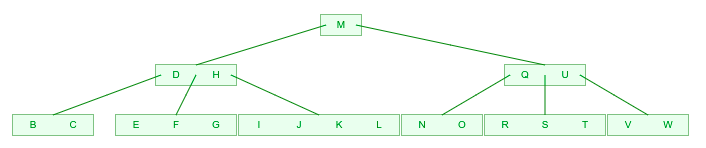
\includegraphics[width=\linewidth]{tree_2.png}
\end{figure}

\begin{figure}[H]
    \centering
    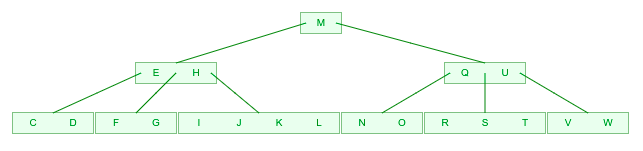
\includegraphics[width=\linewidth]{tree_3.png}
\end{figure}

\begin{figure}[H]
    \centering
    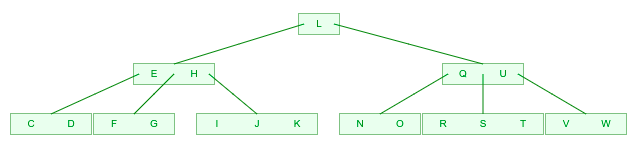
\includegraphics[width=\linewidth]{tree_4.png}
\end{figure}

\begin{figure}[H]
    \centering
    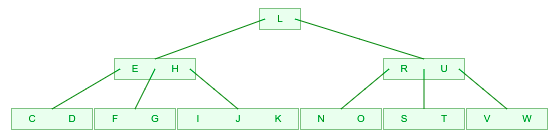
\includegraphics[width=\linewidth]{tree_5.png}
\end{figure}

\begin{figure}[H]
    \centering
    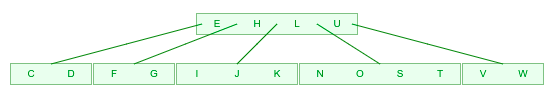
\includegraphics[width=\linewidth]{tree_6.png}
\end{figure}
